\documentclass[../main.tex]{subfiles}
\begin{document}
	
	\chapter{Álgebra Vetorial e Geometria Analítica}
	Para iniciar os estudos de Álgebra Linear, é interessante apresentar, inicialmente, conceitos básicos para visualizar e estruturar o conhecimento. Nesse sentido, entender vetores na perspectiva geométrica, ou seja, no plano ($\mathbb{R}^2$) ou no espaço ($\mathbb{R}^3$), é mais intuitivo em um primeiro contato. Nos próximos capítulos, em especial no capítulo 3, a definição de vetores será ampliada para outros espaços vetoriais, com um maior nível de abstração.
	
	\section{Álgebra Vetorial}
		\begin{definicao}
			\azul{Vetores (geometricamente)} são objetos matemáticos que possuem módulo, direção e sentido.
			
			Usualmente, um vetor é representado por segmentos de retas orientados equipolentes, ou seja, que apresentam mesmo tamanho, direção e sentido.
			\begin{center}
				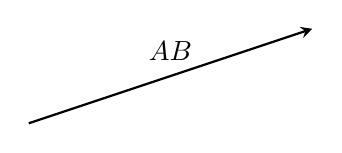
\begin{tikzpicture}[scale=1.2, >=stealth]
					\draw[thick] [->] (0,0) -- (3,1) node[midway, above=2pt] {$\vv{AB}$};
				\end{tikzpicture}
			\end{center}
		\end{definicao}
		Note que, pela definição, um vetor não possui "origem fixa" e pode ser representado por diferentes segmentos de reta orientados.
		\begin{definicao}
			Sejam $u$ e $v$ vetores representados por $\vv{AB}$ e $\vv{BC}$, respectivamente. A \azul{soma de vetores} $u+v$ é definida como o vetor representado pelo segmento de reta orientado $\vv{AC}$  
			\begin{center}
				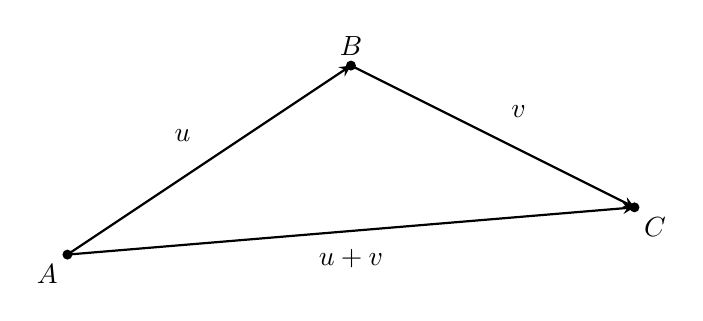
\begin{tikzpicture}[scale=1.2, >=stealth]
					% Pontos
					\coordinate (A) at (0,0);
					\coordinate (B) at (3,2);
					\coordinate (C) at (6,0.5);
					
					% Lados com setas
					\draw[thick, ->] (A) -- (B) node[midway, above left=3pt] {$u$};
					\draw[thick, ->] (B) -- (C) node[midway, above right=3pt] {$v$};
					\draw[thick, ->] (A) -- (C) node[midway, below=3pt] {$u+v$};
					
					% Pontos marcados
					\fill (A) circle (1.5pt) node[below left] {$A$};
					\fill (B) circle (1.5pt) node[above] {$B$};
					\fill (C) circle (1.5pt) node[below right] {$C$};
				\end{tikzpicture}
			\end{center}
		\end{definicao}
		
	\section{Geometria Analítica}
	\section{Matrizes como Vetores}
	
\end{document}
